%; whizzy paragraph -pdf xpdf -latex ./whizzypdfptex.sh
%; whizzy-paragraph "^\\\\begin{frame}"
% latex beamer presentation.
% platex, latex-beamer $B$G%3%s%Q%$%k$9$k$3$H$rA[Dj!#(B 

%     Tokyo Debian Meeting resources
%     Copyright (C) 2009 Junichi Uekawa

%     This program is free software; you can redistribute it and/or modify
%     it under the terms of the GNU General Public License as published by
%     the Free Software Foundation; either version 2 of the License, or
%     (at your option) any later version.

%     This program is distributed in the hope that it will be useful,
%     but WITHOUT ANY WARRANTY; without even the implied warranty of
%     MERCHANTABILITY or FITNESS FOR A PARTICULAR PURPOSE.  See the
%     GNU General Public License for more details.

%     You should have received a copy of the GNU General Public License
%     along with this program; if not, write to the Free Software
%     Foundation, Inc., 51 Franklin St, Fifth Floor, Boston, MA  02110-1301 USA

\documentclass[cjk,dvipdfm,12pt]{beamer}
\usetheme{Tokyo}
\usepackage{monthlypresentation}

%  preview (shell-command (concat "evince " (replace-regexp-in-string "tex$" "pdf"(buffer-file-name)) "&"))
%  presentation (shell-command (concat "xpdf -fullscreen " (replace-regexp-in-string "tex$" "pdf"(buffer-file-name)) "&"))
%  presentation (shell-command (concat "evince " (replace-regexp-in-string "tex$" "pdf"(buffer-file-name)) "&"))
%  presentation (shell-command (concat "evince " (replace-regexp-in-string "tex$" "pdf"(buffer-file-name)) "&"))

%http://www.naney.org/diki/dk/hyperref.html
%$BF|K\8l(BEUC$B7O4D6-$N;~(B
\AtBeginDvi{\special{pdf:tounicode EUC-UCS2}}
%$B%7%U%H(BJIS$B7O4D6-$N;~(B
%\AtBeginDvi{\special{pdf:tounicode 90ms-RKSJ-UCS2}}

\title{$BEl5~%(%j%"(B Debian $BJY6/2q(B}
\subtitle{$B;qNA(B}
\author{$B4d>>(B $B?.MN(B iwamatsu@debian.or.jp\\IRC nick: iwamatsu}
\date{2009$BG/(B2$B7n(B21$BF|(B}
\logo{
\includegraphics[width=8cm]{image200607/openlogo-light.eps}}

\begin{document}

\frame{\titlepage{}}

\emtext{$B@_1D=`Hw$K$46(NO$/$@$5$$(B}

\section{}
\begin{frame}
 \frametitle{Agenda}
\begin{minipage}[t]{0.45\hsize}
  \begin{itemize}
  \item $BCm0U;v9`(B
	\begin{itemize}
	 \item $BFC$K$J$7(B
	\end{itemize}
  \item $B:G6a$N(BDebian$B4XO"$N%$%Y%s%H(B
	\begin{itemize}
	 \item $BA02s$NJY6/2q(B
	\end{itemize}
 \end{itemize}
\end{minipage} 
\begin{minipage}[t]{0.45\hsize}
 \begin{itemize}
  \item Debian $B%Q%C%1!<%8%s%0%O%s%:%*%s(B
 \end{itemize}
\end{minipage}
\end{frame}

\section{$B:G6a(B}

\begin{frame}
 \frametitle{2009$BG/(B01$B7n(B}
\begin{minipage}[t]{0.45\hsize}
  \begin{itemize}
  \item $BCm0U;v9`(B
	\begin{itemize}
	 \item $B0{?)6X;_(B
	 \item $B@/<#(B/$B=!65(B/$B1DMx3hF06X;_(B
	 \item ustream $B$K$F;n83%9%H%j!<%_%s%0Cf(B
	\end{itemize}
  \item $B:G6a$N(BDebian$B4XO"$N%$%Y%s%H(B
	\begin{itemize}
  \item Lenny release
  \item Linux Consortium 10 Years Event !!
$B!!!!(B\item Debian $B%O%C%/%+%U%'3+;O(B
	\end{itemize}
 \end{itemize}
\end{minipage} 
\begin{minipage}[t]{0.45\hsize}
 \begin{itemize}
  \item Debian$B$N(B2009$BG/$NM=Dj$r9M$($k(B
  \item $BE_5Y$_$N=IBjH/I=(B
 \end{itemize}
\end{minipage}
\end{frame}

\begin{frame}{2009$BG/7W2h(B}

{\scriptsize
 \begin{enumerate}
  \item $B?7G/$N4k2h(B ($B$"$s$5$s$V$k2.7&3+:E(B)
  \item OSC Tokyo
  \item Debian Lisp$B4D6-%O%C%/!"8&5f<<$N%=%U%H%&%'%"$r(BDebian$B%Q%C%1!<%8$K(B
	$B$9$k!#(B
  \item Git Handson ($B4d>>(B)($B$"$s$5$s$V$k2.7&(B?)
  \item $B2H(BDebian$B%5!<%P(B vs $B?&>l$N%M%C%H%o!<%/(B($B@iBeED6hETN)?^=q4[(B?\footnote{\url{http://www.library.chiyoda.tokyo.jp/}})
  \item Asterisk ($BEl5~Bg3X(B?)
  \item $B%9%Z%$%s$K$F3+:E(B
  \item Debconf$BJs9p2q(B
  \item OSC Fall?
  \item udev + HAL
  \item 3D graphics $B3+H/(B 
  \item Debian $B%5!<%P(B+VMware + $B3F<o(BOS$B!"(B
	$BB>$N2>A[2=%D!<%k(B(vserver etc.)$B!"(B
	$BK:G/2q(B
 \end{enumerate}
}
\end{frame}

\emtext{Lenny release}

\begin{frame}{Lenny release}
$B$a$G$?$/(B2009$BG/(B02$B7n(B14$BF|(B(UTC)$B$K(B Debian GNU/Linux 5.0($B%3!<%I%M!<%`(B Lenny)$B$,(B
 $B%j%j!<%9$5$l$^$7$?!#3+H/$K4X$o$C$?J}!9!"$*Hh$l$5$^$G$7$?!#(B
\end{frame}

\emtext{Debian $B%Q%C%1!<%8%s%0%O%s%:%*%s(B}
\begin{frame}{$BK\F|$NL\E*(B}
Debian$B%Q%C%1!<%82=$5$l$F$$$J$$%=%U%H%&%'%"$r%Q%C%1!<%82=$7$F!"(B
$B%S%k%I%F%9%H$H%Q%C%1!<%8$NJQ99$^$G$rBN83$7$^$9!#(B
$B$H$3$m$I$3$m$K%H%i%C%W$,$"$k$N$GCm0U$7$^$7$g$&!#(B
\end{frame}

\begin{frame}{$BK\F|$NN.$l(B}
\begin{enumerate}
\item $B9V;U>R2p(B
\item $B:n6H$r;O$a$kA0$NA0=`Hw(B
\item $B%=%U%H%&%'%"$N%3%s%Q%$%k(B
\item $B%Q%C%1!<%8$N?w7A(B
\item CDBS
\item debian$B%G%#%l%/%H%j0J2<%U%!%$%k$NJT=8(B
\item $B%Q%C%1!<%8$N%S%k%I(B
\item $B%Q%C%1!<%8$N%$%s%9%H!<%k(B
\item $B%Q%C%1!<%8$N%S%k%I%F%9%H(B
\item $B%Q%C%1!<%8$N%$%s%9%H!<%k(B/$B%"%s%$%s%9%H!<%k%F%9%H(B
\item $B%W%m%0%i%`$NJT=8(B
\item $B<A5?1~Ez(B
\end{enumerate}
\end{frame}

\emtext{$B9V;U>R2p(B}
\begin{frame}{$B9V;U>R2p(B}
\begin{itemize}
\item $B4d>>(B $B?.MN(B

$B;d!#(BDebian Maintainer$B!#(BDebian JP project $BI{2qD9!"%+!<%M%k3+H/$H$+$=(B
 $B$NB>=t!9!#(B
\item Debian JP Project $BM-;V(B

$B$=$NJU$N$=$l$C$]$$?M$?$A!#$=$C$A7O$N%W%m$NJ}$G$9!#(B
\end{itemize}
\end{frame}

\emtext{$BA02s$N%O%s%:%*%s(B}
\begin{frame}
\begin{itemize}
\item $B5nG/$N(BOSC 2008 TOKYO Spring $B$G3+:E(B
\item 39$BL>;22C(B
\item $BLdBjE@(B
\begin{enumerate}
\item $B9V;U$,0l?M$@$C$?(B
\item vi $B$,;H$($J$$?M$,$$$?(B
\item $BOC$K$D$$$F$3$l$J$$?M$,$$$?(B
\item $B%O%s%:%*%s2q>l$N%M%C%H%o!<%/$G%H%i%V%k$,$"$C$?(B
\item $B;~4V$,B-$j$J$+$C$?(B
\end{enumerate}
\end{itemize}
\end{frame}

\begin{frame}
\begin{itemize}
\item $BBP:v(B
\begin{enumerate}
\item $B9V;U$,0l?M$@$C$?(B

TA $B$rIU$1$^$7$?!#(B
\item vi $B$,;H$($J$$?M$,$$$?(B

vi $B0J30$N%(%G%#%?$rDI2C$7$^$7$?!#$^$?!"(BX$B>e$G9T$&$h$&$K$7$^$7$?!#(B
\item $BOC$K$D$$$F$3$l$J$$?M$,$$$?(B

$B%F%-%9%H$rMQ0U$7$^$7$?!#(B
\item $B%O%s%:%*%s2q>l$N%M%C%H%o!<%/$G%H%i%V%k$,$"$C$?(B

$B%M%C%H%o!<%/$r;H$o$J$$$h$&$K$7$^$7$?!#(B
\item $B;~4V$,B-$j$J$+$C$?(B

2$B;~4VOH$r<h$j$^$7$?!#(B
\end{enumerate}
\end{itemize}
\end{frame}

\emtext{$B$*4j$$(B}
\begin{frame}{$B$*4j$$(B}
\begin{itemize}
\item $B:$$C$?;v$,$"$C$?$i(B{\bf TA}$B$N?M$KJ9$$$F$/$@$5$$!#(B
\item $BNY$N?M$,:$$C$F$$$?$i=u$1$F>e$2$F$/$@$5$$!#$46(NO$*4j$$$7$^$9!#(B
\item $B%H%i%C%W$,J,$+$C$F$b$D$C$3$^$J$$$h$&$K$7$F$/$@$5$$!#$?$V$s$=$l$O(B
      {\bf $B%O%s%:%*%s$N%M%?(B}$B$J$N$G!"$h$m$7$/$*4j$$$7$^$9!#(B
\end{itemize}
\end{frame}


\emtext{$B;vA0=`Hw(B}
\begin{frame}{$B5-9f$N@bL@(B}

\begin{itemize}
\item {\bf \$} $B$,IU$$$F$$$k>l9g$O!"%3%s%=!<%k$+$i$NF~NO$r0UL#$7$^$9!#(B{\bf \$}$B$OF~NO$;$:$K(B
$B%3%^%s%I$rF~NO$7$F$/$@$5$$!#(B

\item $B%3%^%s%I%i%$%s$d%U%!%$%k$NCf?H$G(B{\bf \textbackslash}$B$,=q$+$l$F$$$k>l=j$O9T$,B3$$$F(B
$B$$$k;v$r0UL#$7$^$9!#F~NO$7$J$$$G$/$@$5$$!#(B 

\item {\bf ...}$B$O>JN,$r0UL#$7$^$9!#<B:]$K$OD9$$=PNO$,$"$k>l9g$K>JN,$7$F$$$k>l(B
$B9g$KMxMQ$7$F$$$^$9!#(B
\end{itemize}

\end{frame}


\begin{frame}{$B%(%G%#%?(B}
$BK\%O%s%:%*%s$G$O!"%(%G%#%?$H$7$F(B{\bf vi}$B$*$h$S(B{\bf mousepad}$B$r;H$($k$h$&$K$7$F$$(B
$B$^$9!#(B{\bf vi}$B$,;H$($J$$?M$O!"(B{\bf mousepad}$B$r;H$C$F$/$@$5$$!#(B
\end{frame}

\begin{frame}{$B%k!<%H8"8B$K$D$$$F(B}
$BK\%O%s%:%*%s$G$O!"(Broot$B8"8B$r;H$C$?:n6H$r9T$&>l9g$,$"$j$^$9!#(B
$B$=$N>l9g$K$O(B {\bf sudo}$B%3%^%s%I$r;H$C$F:n6H$r$7$^$9!#(B{\bf sudo}$B%3%^%s%I$,I,MW$J>l(B
$B9g$K$O%3%^%s%I%i%$%s$N@bL@$N$H$3$m$K(B{\bf sudo}$B$r;XDj$7$F$$$^$9!#(B
\end{frame}

%\emtext{$BA0=`Hw(B}
 
\begin{frame}[containsverbatim]{$B%Q%C%1!<%8%a%s%F%JL>$N@_Dj(B}
$B%Q%C%1!<%8%a%s%F%J$NL>A0$H%a!<%k%"%I%l%9$r4D6-JQ?t$K@_Dj$7$^$9!#(B
$BE,Ev$J$G%(%G%#%?$r;H$C$F!"(B{\bf /home/user/.bashrc} $B$K0J2<$NNc$N$h$&$KJQ(B
$B99$7$FJ]B8$7$F$/$@$5$$!#3F9`L\$K$O<+J,$NL>A0$H%a!<%k%"%I%l%9$r$$$l$F$/$@(B
$B$5$$!#(B
\begin{commandline}
export DEBFULLNAME="Nobuhiro Iwamatsu"
export DEBEMAIL=iwamatsu@nigauri.org
\end{commandline}
\end{frame}

\begin{frame}[containsverbatim]
$BJ]B8$G$-$?$i!"%?!<%_%J%k$r5/F0$7!"(B
\begin{commandline}
$ source ~/.bashrc
\end{commandline}
$B$r<B9T$7$F$/$@$5$$!#(B
\end{frame}


\begin{frame}[containsverbatim]{web$B%5!<%P$NN)$A>e$2(B}
$B%3%s%=!<%k$+$i0J2<$N%3%^%s%I$r<B9T$7$F$/$@$5$$!#(B
\begin{commandline}
$ sudo ruby1.8 ./tools/web.rb
\end{commandline}
\end{frame}

\begin{frame}[containsverbatim]{apt-line$B$NJQ99(B}
$B%(%G%#%?$r;H$$!"(B{\bf /etc/apt/sources.list}$B%U%!%$%k$r0J2<$N$h$&$KJQ99$7$F$/$@$5$$!#(B
apt-line $B$,=q$+$l$F$$$^$9$,!":o=|$7$F$/$@$5$$!#(B
\begin{commandline}
deb http://localhost/debian lenny main
\end{commandline}
\end{frame}


\begin{frame}[containsverbatim]{$B%j%]%8%H%j>pJs$N%"%C%W%G!<%H(B}
$B%j%]%8%H%j$N%"%C%W%G!<%H$r9T$$$^$9!#(B
\begin{commandline}
$ sudo apt-get update
\end{commandline}
\end{frame}

\begin{frame}[containsverbatim]{/tmp $B$N%^%&%s%H%*%W%7%g%s$NJQ99(B}
{\bf /tmp}$B$r(B{\bf nodev}$B%*%W%7%g%s$J$7$G(B{\bf remount}$B$7$^$9!#(B
$B0J2<$N$h$&$K<B9T$7$^$9!#(B
\begin{commandline}
sudo mount -o remount,dev /tmp
\end{commandline}
\end{frame}

\begin{frame}[containsverbatim]{$B:#2s$N%5%s%W%k(B}
$B:#2s$O!"(B{\bf cwidget}$B$r;H$C$?%5%s%W%k%W%m%0%i%`(B
{\bf /live/image/osc/data/hello-cwidget-0.1.tar.gz}
$B$rMQ0U$7$^$7$?!#(B
$B$3$N%5%s%W%k%W%m%0%i%`$r(BDebian$B%Q%C%1!<%82=$7$^$9!#(B
{\bf /live/image/osc/data}$B%G%#%l%/%H%j$K%=!<%9%U%!%$%k$,$"$k$N$G!"%[!<%`%G%#%l%/%H%j$KE83+$7$^$9!#(B
\begin{commandline}
$ cd
$ tar -xzf /live/image/osc/data/hello-cwidget-0.1.tar.gz
\end{commandline}

$B$3$N%=%U%H%&%'%"$O(B C++ $B$G5-=R$5$l$F$*$j!"%3%s%Q%$%k$KI,MW$J%i%$%V(B
$B%i%j$d%=%U%H%&%'%"$,%$%s%9%H!<%k$5$l$F$$$k>l9g$K$O!"(B./configure ; make ;
make install $B$G%3%s%Q%$%k$*$h$S%$%s%9%H!<%k$^$G$,$G$-$k$h$&$K$J$C$F$$$^(B
$B$9!#(B
\end{frame}

\emtext{$B%Q%C%1!<%8%s%02=3+;O(B}
\begin{frame}{$B%=!<%9$rFI$s$G$_$k(B}
$BF0:n$7$J$$%W%m%0%i%`$r%Q%C%1!<(B
$B%82=$7$F$b$7$g$&$,$J$$$N$G!"@h$K$I$N$h$&$J%=%U%H%&%'%"$J$N$+M}2r$9$k$?$a(B
$B$K$b%Q%C%1!<%8%s%02=$9$kA0$K%=!<%9%3!<%I$rFI$s$G!"%=%U%H%&%'%"$NCf?H$rM}(B
$B2r$7$FCV$-$^$7$g$&!#(B
\end{frame}

\begin{frame}[containsverbatim]{$B$H$j$"$($:!"%3%s%Q%$%k$7$F$_$k(B}
$BF0$+$J$$%W%m%0%i%`$r%Q%C%1!<%82=$7$F$b$7$g$&$,$J$$$N$G!"F0:n3NG'$r$7$^$9!#(B
$B$^$:$O:GDc8B%3%s%Q%$%k$KI,MW$J%Q%C%1!<%8$r%$%s%9%H!<%k$9$kI,MW(B
$B$,$"$j$^$9!#$=$l$,(B{\bf build-essential}$B%Q%C%1!<%8$G$9!#$3$l$O!"%Q%C%1!<(B
$B%82=$N>l9g$K$bI,MW$G$9!#0J2<$N$h$&$K<B9T$7!"%$%s%9%H!<%k$7$^$9!#(B
\begin{commandline}
$ sudo apt-get install build-essential
\end{commandline}
\end{frame}

\begin{frame}[containsverbatim]
$B@h$[$I2rE`$7$?%G%#%l%/%H%j$K0\F0$7$^$9!#0\F0$7$?$i!"(B{\bf configure}$B$r<B(B
$B9T$7$^$9!#(B
\begin{commandline}
$ cd hello-cwidget-0.1
$ ./configure
...
Alternatively, you may set the environment variables \
SIGC_CFLAGS
and SIGC_LIBS to avoid the need to call pkg-config.
See the pkg-config man page for more details.
...
\end{commandline}
$B<B9T$9$k$H!"%(%i!<$K$J$j$^$9!#(B
$B%(%i!<$O(B pkg-config $B$H(B SIGC\_CFLAGS / SIGC\_LIBS $B$K$h$k$b$N$N$h$&$G$9!#(B
\end{frame}

\begin{frame}[containsverbatim]
{\bf pkg-config} $B$O$I$3$K$"$k$N$+!"D4$Y$F$_$^$9!#(B
\begin{commandline}
$ which pkg-config
\end{commandline}

$B%$%s%9%H!<%k$5$l$F$$$J$$$h$&$G$9!#(B{\bf pkg-config}$B$O$I$N%Q%C%1!<%8$GDs6!(B
 $B$5$l$F$$$k$N$G$7$g$&$+!#(B
\end{frame}

\begin{frame}[containsverbatim]{$BI,MW$J%U%!%$%k$rC5$9(B}
Debian$B$GFCDj$N%U%!%$%k$,Ds6!$5$l$F$$$k%Q%C%1!<%8$rC5$9>l9g$K$O!"(B
{\bf apt-file}$B$rMxMQ$7$^$9!#0J2<$N$h$&$K<B9T$7!"%$%s%9%H!<%k$7$^$9!#(B
\begin{commandline}
$ sudo apt-get install apt-file
\end{commandline}
$BDL>o$O!"(B $B$3$N8e!"(B{\bf apt-file update}$B$r<B9T$7!"%U%!%$%k>pJs%G!<%?$r<hF@$7$^$9$,!"(B
$B4{$K(BLive-CD$B$KF~$l$F$$$k$N$G>JN,$7$^$9!#(B
\end{frame}

\begin{frame}[containsverbatim]
$B%U%!%$%k$rC5$9$K$O0J2<$N$h$&$K<B9T$7$^$9!#(B
\begin{commandline}
$ apt-file search pkg-config
...
nant: /usr/share/doc/nant/help/functions/pkg-config.\
     is-max-version.html
pkg-config: /usr/bin/pkg-config
pkg-config: /usr/share/doc/pkg-config/AUTHORS
...
\end{commandline}
$B<B9T$9$k$H!";XDj$7$?%U%!%$%k$rDs6!$7$F$$$k%Q%C%1!<%8L>$,=PNO$5$l$^$9!#(B
$B=PNO$5$l$?%Q%C%1!<%8$r%$%s%9%H!<%k$7$^$9!#(B

\begin{commandline}
$ sudo apt-get install pkg-config
\end{commandline}
\end{frame}

\begin{frame}[containsverbatim]
$B:FEY(B{\bf configure}$B$r<B9T$7$F$_$^$7$g$&!#(B
\begin{commandline}
$ ./configure
...
No package 'sigc++-2.0' found

Consider adjusting the PKG_CONFIG_PATH environment variable if you
installed software in a non-standard prefix.
...
\end{commandline}
$B$^$@B-$j$J$$%Q%C%1!<%8$,$"$k$h$&$G$9!#@h$[$I$HF1$8$h$&$K(B{\bf apt-file}$B$r(B
$BMxMQ$7$F8!:w$7!"%$%s%9%H!<%k$7$^$9!#(B
\end{frame}

\begin{frame}[containsverbatim]
\begin{commandline}
$ apt-file search sigc++-2.0.pc
libsigc++-2.0-dev: /usr/lib/pkgconfig/sigc++-2.0.pc
$ sudo apt-get install libsigc++-2.0-dev 
\end{commandline}
$B:FEY(B configure $B$r<B9T$7$^$9!#(B
\begin{commandline}
$ ./configure
...
checking for CWIDGET... configure: error: Package \
  requirements(cwidget) were not met:

No package 'cwidget' found

Consider adjusting the PKG_CONFIG_PATH environment variable \
if you
installed software in a non-standard prefix.
...
\end{commandline}
$B%(%i!<$K$J$j$^$9!#$^$@B-$j$J$$$h$&$J$N$G!":FEY8!:w$7$F%$%s%9%H!<%k$7$^$9!#(B
\end{frame}

\begin{frame}[containsverbatim]
\begin{commandline}
$ apt-file search cwidget.pc
libcwidget-dev: /usr/lib/pkgconfig/cwidget.pc
$ sudo apt-get install libcwidget-dev
\end{commandline}

\begin{commandline}
./configure
...
config.status: WARNING:  Makefile.in seems to ignore the \
   --datarootdir setting
config.status: creating src/Makefile
config.status: WARNING:  src/Makefile.in seems to ignore the \
  --datarootdir setting
config.status: creating config.h
\end{commandline}
\end{frame}

\begin{frame}[containsverbatim]

{\bf configure}$B$,@5>o$K=*N;$7$^$7$?!#=*N;$9$k$H!"(B{\bf Makefile}$B$,(B
$B:n@.$5$l$F$$$^$9!#(B{\bf make}$B$r<B9T$7!"%3%s%Q%$%k$7$^$9!#(B
\end{frame}

\begin{frame}[containsverbatim]
\begin{commandline}
$ make
...
make[1]: $B%G%#%l%/%H%j(B `/home/user/hello-cwidget-0.1' \
$B$KF~$j$^$9(B
Making all in src
make[2]: $B%G%#%l%/%H%j(B `/home/user/hello-cwidget-0.1/src' \
$B$KF~$j$^$9(B
g++ -DHAVE_CONFIG_H -I. -I. -I..     -g -O2 -I/usr/ \
include/sigc++-2.0 \
-I/usr/lib/sigc++-2.0/include   -I/usr/lib/cwidget
 -I/usr/include/sigc++-2.0  -I/usr/lib/sigc++-2.0/include \
 -c hello.cc
g++  -g -O2 -I/usr/include/sigc++-2.0 -I/usr/lib/ \
sigc++-2.0/include   \
-I/usr/lib/cwidget -I/usr/include/sigc++-2.0
-I/usr/lib/sigc++-2.0/include \
-o hello  hello.o  -lsigc-2.0   -lcwidget -lncursesw \
-lsigc-2.0  
make[2]: $B%G%#%l%/%H%j(B `/home/user/hello-cwidget-0.1/src' \
$B$+$i=P$^$9(B
make[2]: $B%G%#%l%/%H%j(B `/home/user/hello-cwidget-0.1' $B$KF~$j$^$9(B
make[2]: $B%G%#%l%/%H%j(B `/home/user/hello-cwidget-0.1' $B$+$i=P$^$9(B
make[1]: $B%G%#%l%/%H%j(B `/home/user/hello-cwidget-0.1' $B$+$i=P$^$9(B
\end{commandline}
\end{frame}

\begin{frame}[containsverbatim]
$B%3%s%Q%$%k$b@5>o$K=*N;$7$?$N$G!";n$7$K<B9T$7$F$_$^$9!#(B
\begin{commandline}
$ ./src/hello
\end{commandline}
\end{frame}

\begin{frame}[containsverbatim]
\begin{center}
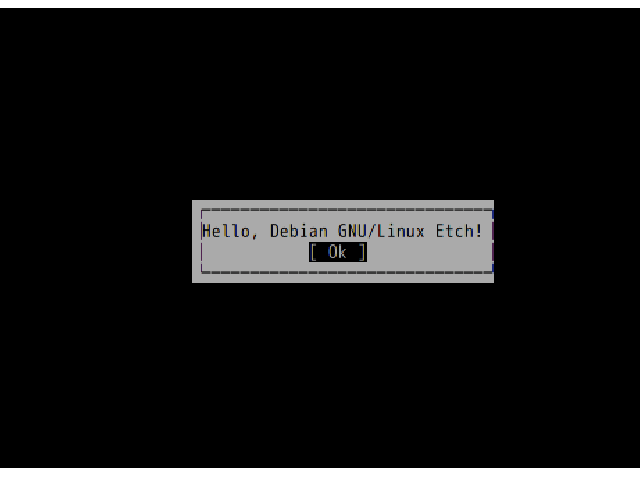
\includegraphics[width=8cm]{image200902/hello-cw.png}
\end{center}

\end{frame}

\begin{frame}[containsverbatim]
$B$3$3$^$G$O%5%s%W%k%W%m%0%i%`$NF0:n3NG'$G$9!#F0:n$7$J$$%W%m%0%i%`$r%Q%C%1!<(B
$B%82=$7$F$b$7$g$&$,$J$$$N$G!"@h$K$I$N$h$&$J%=%U%H%&%'%"$J$N$+M}2r$9$k$?$a(B
$B$K$b%Q%C%1!<%8%s%02=$9$kA0$K%=!<%9%3!<%IEy$rFI$s$G$*$/$3$H$r$*4+$a$7$^$9!#(B
\end{frame}

\emtext{$B%Q%C%1!<%8$N?w7A(B}

\begin{frame}[containsverbatim]

{\bf dh\_make}$B%3%^%s%I$G%Q%C%1!<%8$N?w7A$r:n@.$9$k$3$H$,$G$-$^$9!#(B
{\bf dh\_make}$B$O!"(B{\bf dh-make}$B%Q%C%1!<%8$GDs6!$5$l$F$$$^$9!#(B
$B0J2<$N%3%^%s%I$r<B9T$7!"%$%s%9%H!<%k$7$^$9!#(B
\begin{commandline}
$ sudo apt-get install dh-make
\end{commandline}
\end{frame}

\begin{frame}[containsverbatim]

$B?w7A$N:n@.$O0J2<$N%3%^%s%I$r<B9T$7$^$9!#(B
\begin{commandline}
$ dh_make --createorig -s
\end{commandline}
{\bf --createorig}$B%*%W%7%g%s$O%*%j%8%J%k%=!<%9%3!<%I$N(Btar.gz$B%$%a!<%8$r9=C[$7(B
  $B$^$9!#(B $B:#2s$O%7%s%0%k%P%$%J%j%Q%C%1!<%8!J0l$D$N%=!<%9%3!<%I$+$i0l$D$N(B
  $B%P%$%J%j%Q%C%1!<%8$,:n@.$5$l$k!K$J$N$G(B{\bf -s} $B$r;XDj$7$^$9!#<B9T$9$k$H0J2<(B
  $B$N$h$&$J%a%C%;!<%8$,I=<($5$l$k$N$G!"(BEnter$B%-!<$r2!$7$^$9!#(B
\begin{commandline}
Maintainer name : Nobuhiro Iwamatsu
Email-Address   : iwamatsu@nigauri.org 
Date            : Sun, 15 Feb 2009 23:51:58 +0900
Package Name    : hello-cwidget
Version         : 0.1
License         : blank
Using dpatch    : no
Using quilt     : no
Type of Package : Single
Hit <enter> to confirm: 
\end{commandline}
\end{frame}


\begin{frame}[containsverbatim]{debian$B%G%#%l%/%H%j(B}
$B$&$^$/F0:n$9$k$H!"(B{\bf debian$B%G%#%l%/%H%j(B}$B$,:n@.$5$l!"$3$NCf$K?w7A$,:n@.$5$l(B
$B$^$9!#%Q%C%1!<%8%a%s%F%J$O$3$N%G%#%l%/%H%j$NCf0J30$O?($j$^$;$s!#(B
\end{frame}

\begin{frame}[containsverbatim]
\begin{commandline}
.
|-- README.Debian  (Debian$B%Q%C%1!<%8$N(B README)
|-- changelog      (Debian$B%Q%C%1!<%8$N%A%'%s%8%m%0(B)
|-- compat         (Debian$B%Q%C%1!<%8$N%P!<%8%g%s(B)
|-- control        (Debian$B%Q%C%1!<%8>pJs(B)
|-- copyright      ($B%3%T!<%i%$%H>pJs(B)
|-- cron.d.ex      (cron $B$r;H$&%Q%C%1!<%8MQ@_Dj%U%!%$%k(B)
|-- dirs           ($B:n@.$9$k%G%#%l%/%H%jL>$r;XDj$9$k(B)
|-- docs           ($B%$%s%9%H!<%k$9$k%I%-%e%a%s%H%U%!%$%k$r;XDj$9$k(B)
|-- emacsen-install.ex (emacs $BMQ@_Dj%U%!%$%k(B)
|-- emacsen-remove.ex  (emacs $BMQ@_Dj%U%!%$%k(B)
|-- emacsen-startup.ex (emacs $BMQ@_Dj%U%!%$%k(B)
|-- hello-cwidget.default.ex (debfonf$BMQ(B)
|-- hello-cwidget.doc-base.EX (doc-base$BMQ(B)
\end{commandline}
\end{frame}

\begin{frame}[containsverbatim]
\begin{commandline}
|-- init.d.ex      (init.d$B$r;H$&%Q%C%1!<%8MQ@_Dj%U%!%$%k(B)
|-- init.d.lsb.ex  (init.d$B$r;H$&%Q%C%1!<%8MQ@_Dj%U%!%$%k(B)
|-- manpage.1.ex   (manpage $B$N?w7A(B)
|-- manpage.sgml.ex(manpage $B$N?w7A(B)
|-- manpage.xml.ex (manpage $B$N?w7A(B)
|-- menu.ex        ($B%a%K%e!<$N?w7A(B)
|-- postinst.ex    (postinst$B%a%s%F%J%U%!%$%k$N?w7A(B)
|-- postrm.ex      (postrm$B%a%s%F%J%U%!%$%k$N?w7A(B)
|-- preinst.ex     (preinst$B%a%s%F%J%U%!%$%k$N?w7A(B)
|-- prerm.ex       (prerm$B%a%s%F%J%U%!%$%k$N?w7A(B)
|-- rules          ($B%Q%C%1!<%8%S%k%I%9%/%j%W%H(B)
`-- watch.ex       ($B%"%C%W%9%H%j!<%`%A%'%C%/MQ%U%!%$%k(B)
\end{commandline}
\end{frame}

\begin{frame}{CDBS}
./configure ; make ; make install $B$G%Q%C%1!<%8$N%3%s%Q%$%k$,$G$-$k(B
$B%=%U%H%&%'%"$O(B cdbs $B$r;H$C$?J}$,MF0W$K(BDebian$B%Q%C%1!<%82=$G$-$^$9!#(B
\end{frame}


\begin{frame}[containsverbatim]{$B0l2s(B hello-cwidget$B%G%#%l%/%H%j$r:o=|$9$k(B}
$B8=>u$G$O@h$[$I$N(B{\bf dh\_make}$B$N7k2L$,;D$C$F$$$k$N$G0l2s!"%5%s%W%k%W%m%0(B
$B%i%`$N%G%#%l%/%H%j$4$H:o=|$7!":FEYE83+$7$^$9!#(B
\begin{commandline}
$ cd 
$ rm -rf hello-cwidget-0.1.*
$ tar -xzf /live/image/osc/data/hello-cwidget-0.1.tar.gz
$ cd hello-cwidget-0.1
\end{commandline}
\end{frame}

\begin{frame}[containsverbatim]{dh\_make$B$r<B9T$7!"%Q%C%1!<%8$N?w7A$r:n@.$9$k(B}

{\bf CDBS}$B$r;H$&(BDebian$B%Q%C%1!<%8$N?w7A:n@.$O0J2<$N%3%^%s%I$r<B9T$7$^$9!#(B
\begin{commandline}
$ dh_make --createorig -b
\end{commandline}
{\bf -b}$B%*%W%7%g%s$r;XDj$9$k$H!"(BCDBS $B$r;H$C$??w7A$r:n@.$7$^$9!#(B
\end{frame}

\begin{frame}[containsverbatim]
\begin{commandline}
Maintainer name : Nobuhiro Iwamatsu
Email-Address   : iwamatsu@nigauri.org 
Date            : Sun, 15 Feb 2009 23:51:58 +0900
Package Name    : hello-cwidget
Version         : 0.1
License         : blank
Using dpatch    : no
Using quilt     : no
Type of Package : cdbs
Hit <enter> to confirm: 
\end{commandline}
\end{frame}

\begin{frame}[containsverbatim]{$BITMW$J%U%!%$%k$N:o=|(B}
$B:#2s$N%Q%C%1!<%82=$KI,MW$G$O$J$$%U%!%$%k$r(B{\bf debian}$B%G%#%l%/%H%j0J2<$+$i:o=|(B
$B$7$^$9!#(B
\begin{commandline}
$ rm -rf debian/*.ex debian/*.EX
\end{commandline}
\end{frame}

\begin{frame}[containsverbatim]{debian/changelog$B%U%!%$%k$NJT=8(B}

{\bf debian/changelog}$B%U%!%$%k$K$O(B{\bf ITP}(Intent To Package)
$B$N%P%0$,4{$K=q$+$l$F$$$k$G:o=|$7$^$9!#0J2<$N$h$&$KJQ99$7$^$9!#(B
\begin{commandline}
hello-cwidget (0.1-1) unstable; urgency=low

  * Initial release.

 -- Nobuhiro Iwamatsu <iwamatsu@nigauri.org> \
                  Wed, 18 Feb 2009 16:31:25 +0000

\end{commandline}
\end{frame}

\begin{frame}[containsverbatim]{debian/copyright$B%U%!%$%k$NJT=8(B}
\begin{commandline}
This package was debianized by Nobuhiro Iwamatsu \ 
                                <iwamatsu@nigauri.org> on
Wed, 18 Feb 2009 16:31:25 +0000.

It was downloaded from <http://www.nigauri.org/~iwamatsu/>

Upstream Author:

    Nobuhiro Iwamatsu <iwamatsu@nigauri.org>

Copyright:

    Copyright (C) 2009 Nobuhiro Iwamatsu <iwamatsu@nigauri.org>

License:

    GPLv2

The Debian packaging is (C) 2009, Nobuhiro Iwamatsu \ 
        <iwamatsu@nigauri.org> and
is licensed under the GPL, see `/usr/share/common-licenses/GPL'.
\end{commandline}
\end{frame}

\begin{frame}[containsverbatim]{debian/control$B%U%!%$%k$NJT=8(B}
\begin{commandline}
Source: hello-cwidget
Section: devel
Priority: extra
Maintainer: Nobuhiro Iwamatsu <iwamatsu@nigauri.org>
Build-Depends: cdbs, debhelper (>= 7), autotools-dev
Standards-Version: 3.8.0
Homepage: http://www.nigauri.org/~iwamatsu/

Package: hello-cwidget
Architecture: any
Depends: ${shlibs:Depends}, ${misc:Depends}
Description: Debian Packaging Hands-on sample program
 This is sample program of Debian Hands-on done with
 OSC2009 TOKYO Spring.
 This is very easy program that uses CWidget.
\end{commandline}
\end{frame}

\begin{frame}[containsverbatim]{$B%Q%C%1!<%8$N%S%k%I(B}

$B%Q%C%1!<%8$N%S%k%I$K$O(B{\bf debuild}$B%3%^%s%I(B $B$r;H$$$^$9!#(B
debuild$B%3%^%s%I$O(B{\bf devscripts}$B%Q%C%1!<%8$GDs6!$5$l$F$$$^$9!#(B
$B$^$?!"$^$@(B {\bf CDBS}$B%Q%C%1!<%8$r%$%s%9%H!<%k$7$F$$$J$$$N$G!"0l=o$K%$%s(B
$B%9%H!<%k$7$^$9!#(B
$B%Q%C%1!<%8$r%$%s%9%H!<%k$7$?$i!"%Q%C%1!<%8$N%S%k%I$r$7$F$_$^$7$g$&!#(B
\begin{commandline}
$ sudo apt-get install devscripts cdbs
$ debuild -us -uc
...
dpkg-buildpackage: full upload (original source is included)
Now running lintian...
W: hello-cwidget: binary-without-manpage usr/bin/hello
W: hello-cwidget: new-package-should-close-itp-bug
Finished running lintian.
\end{commandline}
\end{frame}

\begin{frame}[containsverbatim]{$B%Q%C%1!<%8$N%$%s%9%H!<%k(B}
$B%Q%C%1!<%8$,L5;v%S%k%I$G$-$?$i!"<B:]$K%$%s%9%H!<%k$7$F$_$^$9!#(B
$B%$%s%9%H!<%k$K$O(B dpkg $B%3%^%s%I$r;H$C$F%$%s%9%H!<%k$7$^$9!#%$%s%9%H!<%k$7(B
$B$?$i!"<B:]$KF0$/$+3NG'$7$F$_$^$7$g$&!#(B
\begin{commandline}
$ sudo dpkg -i ../hello-cwidget_0.1-1_i386.deb
$ which hello
$ hello
\end{commandline}
\end{frame}

\begin{frame}{$B%Q%C%1!<%8$N%S%k%I%F%9%H(B}
$B%Q%C%1!<%8$,$G$-$?$"$H$K$O%Q%C%1!<%8$N%F%9%H$r9T$$$^$9!#(B
$B%Q%C%1!<%8$N%S%k%I%F%9%H$K$O(B{\bf pbuilder}$B$r;H$$$^$9!#(B
pbuilder$B$O(BDebian$B$KI,MW$J:GDc8B$N4D6-$+$i%S%k%I$r9T$$!"(B
$B0MB84X78Ey$N%A%'%C%/$r9T$C$F%S%k%I%F%9%H$r9T$&%D!<%k$G$9!#(B
\end{frame}

\begin{frame}[containsverbatim]{pbuilder$B%Q%C%1!<%8$N%$%s%9%H!<%k(B}
\begin{commandline}
$ sudo apt-get install pbuilder
\end{commandline}
\end{frame}

\begin{frame}[containsverbatim]{pbuilder$B4D6-$N9=C[(B}

$B%S%k%I%F%9%H$r9T$&A0$K(Bbase$B%7%9%F%`%$%a!<%8$r9=C[$9$kI,MW$,$"$j$^$9!#(B
$BDL>o$O0J2<$N$h$&$K<B9T$7$^$9$,!"(B
\begin{commandline}
$ sudo pbuilder --create --distribution lenny
\end{commandline}
$B:#2s$O%a%b%j$N@)8B$,$"$k$?$a!"4{$KMQ0U$7$F$"$k(Bbase$B%7%9%F%`%$%a!<%8$rMxMQ(B
$B$7$^$9!#%$%a!<%8$O(B{\bf /live/image/osc/data/base.tgz}$B$K$"$j$^$9!#(B
\end{frame}

\begin{frame}[containsverbatim]{$B%Q%C%1!<%8$N%S%k%I%F%9%H(B}
pbuilder $B$G%F%9%H$9$k>l9g$K$O:n@.$5$l$?%Q%C%1!<%8$N(B{\bf dsc}$B%U%!%$%k$r;XDj$7(B
$B$^$9!#$3$N%U%!%$%k$K$O!"(BDebian$B%Q%C%1!<%8$N9=@.$KI,MW$J%U%!%$%kL>$,=q$+$l(B
$B$F$$$k$N$G!"$=$N>pJs$r85$K:F%S%k%I$r9T$&$3$H$,$G$-$^$9!#(B
$B$^$?!"<B9TA0$K(B{\bf apt-get clean}$B%3%^%s%I$r<B9T$7$F%-%c%C%7%e$r%/%j%"$7(B
$B$F$/$@$5$$!#%a%b%j$,B-$j$J$$$?$a$G$9!#(B
\begin{commandline}
$ cd ..
$ sudo apt-get clean
$ sudo pbuilder --build --distribution lenny \ 
     --basetgz /live/image/osc/data/base.tgz \
     --buildplace /tmp hello-cwidget_0.1-1.dsc
...
\end{commandline}
\end{frame}

\begin{frame}{$B$J$<%(%i!<$K$J$k$N$+(B}
$B@h$[$I$N<j=g$G$d$C$F$b%S%k%I%(%i!<$K$J$j$^$9!#(B
$B$J$<%(%i!<$K$J$k$N$G$7$g$&$+!#9M$($F$_$^$7$g$&!#(B
\end{frame}

\begin{frame}[containsverbatim]{$B%(%i!<$N860x(B}
$B%S%k%I$KI,MW$J%Q%C%1!<%8$,;XDj$5$l$F$$$J$$$?$a$K!"$3$NLdBj$OH/@8$7$^$9!#(B
$B@5$7$$(Bhello-cwidget$B%Q%C%1!<%8$N0MB84X78$r8+$F$_$^$9!#(B
\end{frame}

\begin{frame}
\begin{center}
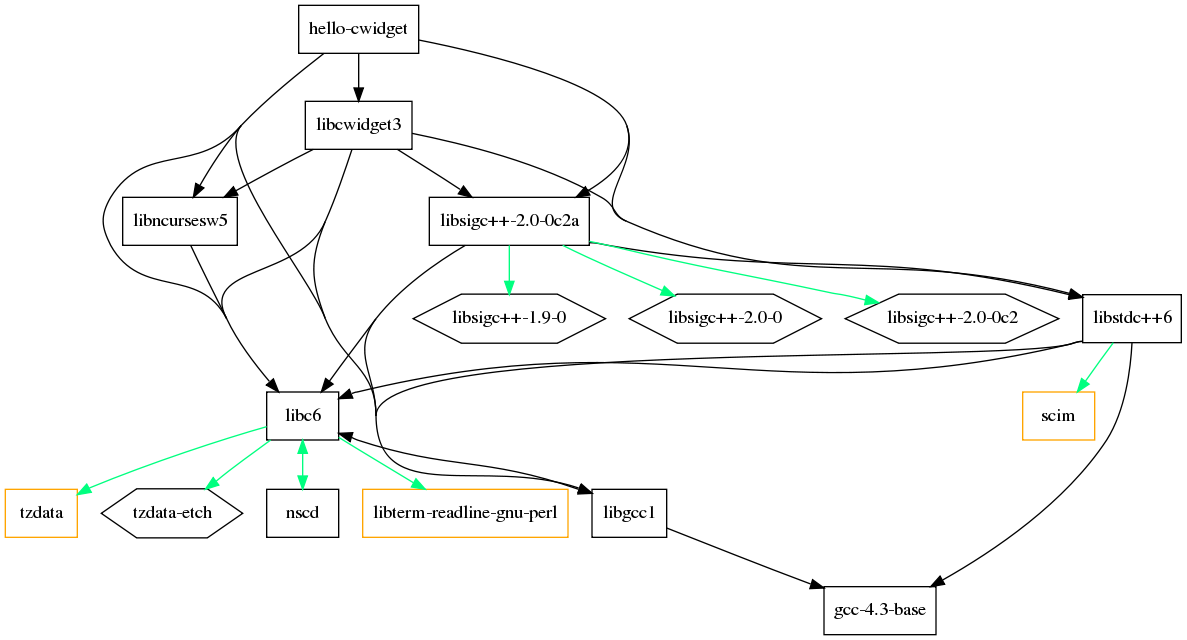
\includegraphics[width=11.5cm]{image200902/cwidget.png}
\end{center}
\end{frame}

\begin{frame}[containsverbatim]
debian/control $B%U%!%$%k$r8+$F$_$^$9!#(B

\begin{commandline}
Source: hello-cwidget
Section: devel
Priority: extra
Maintainer: Nobuhiro Iwamatsu <iwamatsu@nigauri.org>
Build-Depends: cdbs, debhelper (>= 7), autotools-dev
Standards-Version: 3.8.0
Homepage: http://www.nigauri.org/~iwamatsu/

Package: hello-cwidget
Architecture: any
Depends: ${shlibs:Depends}, ${misc:Depends}
Description: Debian Packaging Hands-on sample program
 This is sample program of Debian Hands-on done with
 OSC2009 TOKYO Spring.
 This is very easy program that uses CWidget.
\end{commandline}
\end{frame}


\begin{frame}[containsverbatim]{$B:F%S%k%I%F%9%H(B}
$B%(%i!<$K$J$kM}M3$O@h$K%$%s%9%H!<%k$7$?%Q%C%1!<%8(B{\bf libcwidget-dev}$B$r%Q%C%1!<(B
$B%8%S%k%I;~$N0MB84X78$r5-=R$9$k%U%#!<%k%I(B{\bf Build-Depends}$B$KDI2C$7$F$$(B
$B$J$$$?$a$G$9!#DI2C$7$F!":F%S%k%I$7$F$_$^$9!#(B

debian/control $B%U%!%$%k$r0J2<$N$h$&$K=$@5$7$^$9!#(B

\begin{commandline}
...
Maintainer: Nobuhiro Iwamatsu <iwamatsu@nigauri.org>
Build-Depends: cdbs, debhelper (>= 7), autotools-dev, libcwidget-dev
...
\end{commandline}
\end{frame}

\begin{frame}[containsverbatim]
$B:F%S%k%I$K$O0J2<$N$h$&$K<B9T$7$^$9!#:#EY$O$&$^$/%S%k%I$,$G$-$k$O$:$G$9!#(B
\begin{commandline}
$ sudo pdebuild -- --distribution lenny --basetgz \
 /live/image/osc/data/base.tgz --buildplace /tmp
\end{commandline}
\end{frame}


\begin{frame}{$B%Q%C%1!<%8$N%$%s%9%H!<%k(B/$B%"%s%$%s%9%H!<%k%F%9%H(B}
$B%Q%C%1!<%8$,%S%k%I$G$-$?$@$1$G$O4n$s$G$O$$$1$^$;$s!#%$%s%9%H!<%k(B/$B%"%s%$(B
$B%s%9%H!<%k$N%F%9%H$b9T$$$^$7$g$&!#(B
$B%Q%C%1!<%8$N%$%s%9%H!<%k(B/$B%"%s%$%s%9%H!<%k$N%F%9%H$K$O(B{\bf piuparts}$B%Q%C(B
$B%1!<%8$r;H$$$^$9!#(B
\end{frame}

\begin{frame}[containsverbatim]{piuparts$B$N%$%s%9%H!<%k(B}
$B0J2<$N$h$&$K<B9T$7!"%$%s%9%H!<%k$7$^$9!#(B
\begin{commandline}
$ sudo apt-get install piuparts
\end{commandline}
\end{frame}

\begin{frame}[containsverbatim]{$B%Q%C%1!<%8$N%$%s%9%H!<%k(B/$B%"%s%$%s%9%H!<%k%F%9%H(B}
piuparts$B$b(Bpbuilder$B$HF1MM$K:GDc8B$N4D6-$+$i$N%$%s%9%H!<%k$r%A%'%C%/$7$^$9!#(B
$B$h$C$F!"(Bbase$B%7%9%F%`%$%a!<%8$,I,MW$G$9!#IaCJ$O;XDj$9$kI,MW$O$"$j$^$;$s$,!"(B
$B:#2s$O(B{\bf -b}$B%*%W%7%g%s$rIU$1$F!"(B{\bf /live/image/osc/data/base.tgz}$B$K(B
$B$"$k(Bbase$B%7%9%F%`%$%a!<%8$r;XDj$7$F<B9T$7$^$9!#(B
\begin{commandline}
$ cd ..
$ sudo piuparts -d lenny -b /live/image/osc/data/base.tgz \
   hello-cwidget_0.1-1_i386.deb
...
0m41.9s DEBUG: Removed directory tree at /tmp/tmpHliOKO
0m41.9s INFO: PASS: All tests.
0m41.9s INFO: piuparts run ends.
\end{commandline}
\end{frame}

\begin{frame}{$B%W%m%0%i%`$NJT=8(B}
hello-cwidget$B$r<B9T$7$F!"0cOB46$N$"$kJ}$,$*$i$l$?$H;W$$$^$9!#(B
$B$=$&!"(B{\bf Lenny}$B$,%j%j!<%9$5$l$?$H$$$&$N$K(B{\bf Etch}$B$K$J$C$F$$$^$7$?!#(B
$B$3$l$O$h$/$J$$$N$GJQ99$7$F$_$^$9!#:#2s$O$h$/MxMQ$5$l$F$$$k(B{\bf dpatch}
$B$r;H$C$F@bL@$7$^$9!#(B
\end{frame}

\begin{frame}[containsverbatim]{dpatch$B$N%$%s%9%H!<%k(B}
dpatch$B$r%$%s%9%H!<%k$9$k$K$O!"0J2<$N$h$&$K<B9T$7$^$9!#(B
\begin{commandline}
$ sudo apt-get install dpatch
\end{commandline}
\end{frame}

\begin{frame}[containsverbatim]{dpatch$B$r;H$&$?$a$N=`Hw(B}
dpatch$B$r;H$&A0$K!"(B{\bf debian/rules}$B%U%!%$%k$K(Bdpatch$B$r;H$&$h$&$K@_Dj$9$kI,MW$,(B
$B$"$j$^$9!#(Bdpatch$B$O0l2s!"%Q%C%1!<%8$N>uBV$r=i4|2=$7$F$+$i9T$&$?$a$G$9!#(B
{\bf hello-cwidget-0.1} $B%G%#%l%/%H%j$K0\F0$7$F!"(B{\bf debian/rules}$B$r0J2<$N$h$&$K=$@5$7$^$9!#(B

\begin{commandline}
$ cd  hello-cwidget-0.1
\end{commandline}

\begin{commandline}
#!/usr/bin/make -f

include /usr/share/cdbs/1/rules/debhelper.mk
include /usr/share/cdbs/1/class/autotools.mk
include /usr/share/cdbs/1/rules/dpatch.mk
include /usr/share/dpatch/dpatch.make
\end{commandline}
\end{frame}


\begin{frame}[containsverbatim]{dpatch$B$N<B9T(B}
dpatch$B$O<+%Q%C%1!<%8$r0l2s%3%T!<$7!"(Bdpatch$B4D6-$K0\9T$7$^$9!#(B
$B$=$NCf$GJQ99$7$F!"(Bdpatch$B4D6-$r=*N;$9$k;~$K:9J,$r:n@.$7$^$9!#(B
dpatch$B4D6-$K0\9T$9$k$K$O(B{\bf dpatch-edit-patch}$B%3%^%s%I$K(B
$B:n@.$9$k:9J,$rJ]B8$9$k%U%!%$%kL>$r;XDj$7$F<B9T$7$^$9!#(B
$B0J2<$N$h$&$K<B9T$7$F$/$@$5$$!#(B
\begin{commandline}
$ dpatch-edit-patch 01_change_dist
\end{commandline}
\end{frame}


\begin{frame}[containsverbatim]{$B%U%!%$%k$NJQ99(B}
$B:#2sJQ99$9$k%U%!%$%k$O(B{\bf src/hello.cc}$B$G$9!#(B
$B%(%G%#%?$r5/F0$7!"BP>]$N%U%!%$%k$rJQ99$7$^$9!#(Bmousepad$B$N>l9g$O0J2<$N$h$&(B
$B$K<B9T$7$^$9!#(B
\begin{commandline}
$ mousepad ./src/hello.cc
\end{commandline}
{\bf Etch}$B$NItJ,$r(B{\bf Lenny}$B$KJQ99$7$?$"$H!"J]B8$7$F%(%G%#%?$r(B
$B=*N;$7$^$9!#(B
\end{frame}


\begin{frame}[containsverbatim]{dpatch$B4D6-$r=*N;$9$k(B}
dpatch$B4D6-$r=*N;$9$k$K$O0J2<$N$h$&$K<B9T$7$F$/$@$5$$!#(B
$B<B9T$9$k$H!":9J,$r%U%!%$%k$KJ]B8$7$F(Bdpatch$B4D6-$r=*N;$7$^$9!#(B
\begin{commandline}
$ exit
\end{commandline}
\end{frame}

\begin{frame}[containsverbatim]{$B:n@.$5$l$?:9J,(B(patch)$B$NCf?H(B}
$B:n@.$5$l$?:9J,$O(B\\
{\bf debian/patches/01\_change\_dist.dpatch}
$B$H$7$FJ]B8$5$l$F$$$^$9!#0J2<$N$h$&$JFbMF$K$J$C$F$$$k$O$:$G$9!#(B
\begin{commandline}
#! /bin/sh /usr/share/dpatch/dpatch-run
## 01_change_dist.dpatch by Nobuhiro Iwamatsu <iwamatsu@nigauri.org>
##
## All lines beginning with `## DP:' are a description of the patch.
## DP: No description.

@DPATCH@
diff -urNad hello-cwidget-0.1~/src/hello.cc hello-cwidget-0.1/src/hello.cc
--- hello-cwidget-0.1~/src/hello.cc 2009-02-15 06:56:01.000000000 +0000
+++ hello-cwidget-0.1/src/hello.cc  2009-02-18 16:54:40.668274925 +0000
@@ -26,7 +26,7 @@
    toplevel::init();

    widgets::widget_ref dialog =
-       dialogs::ok(L"Hello, Debian GNU/Linux Etch!",
+       dialogs::ok(L"Hello, Debian GNU/Linux Lenny!",
            util::arg(sigc::ptr_fun(toplevel::exitmain)));

    toplevel::settoplevel(dialog);
\end{commandline}
\end{frame}

\begin{frame}[containsverbatim]
$B%Q%C%A$K$O$J$<$=$N$h$&$J@bL@$r$7$?$N$+!"@bL@$r=q$/I,MW$,$"$j$^$9!#(B
{\bf \#\# DP: No description.}$B$NItJ,$K@bL@$r=q$-$^$9!#(B
$B0J2<$N$h$&$KJQ99$9$k$H$$$$$+$b$7$l$^$;$s!#(B
\begin{commandline}
## DP: Change distributin name from Etch to Lenny.
\end{commandline}
\end{frame}

\begin{frame}[containsverbatim]{$B:n@.$7$?:9J,$r%Q%C%1!<%8$KH?1G$5$;$k(B}
$B:9J,$O:n@.$5$l$^$7$?$,!"$3$N$^$^$G$O%Q%C%1!<%8:n@.;~$K:9J,$,E,MQ$5$l(B
$B$^$;$s!#(Bdpatch$B$r;H$C$F:9J,$r%Q%C%1!<%8$KE,MQ$5$;$k$K$O(B{\bf
debian/patches/00list}$B%U%!%$%k$r:n@.$7!"%Q%C%1!<%8$K(B
$B%Q%C%A$r%U%!%$%k$KNs5s$9$kI,MW$,$"$j$^$9!#(B{\bf debian/patches/00list}$B$r(B
$B0J2<$N$h$&$KJQ99$7$^$9!#(B
\begin{commandline}
01_change_dist.dpatch
\end{commandline}
\end{frame}

\begin{frame}[containsverbatim]{$B:9J,$rE,MQ$7$?%Q%C%1!<%8$r:n@.$9$k(B}
$B:9J,$rE,MQ$7$?%Q%C%1!<%8$r:n@.$9$k$K$ODL>o$N%Q%C%1!<%8:n@.$HJQ$o$j$^$;$s!#(B
{\bf debuild}$B%3%^%s%I$r;H$C$F:n@.$7$^$9!#(B
\begin{commandline}
$ debuild -us -uc
....
\end{commandline}
\end{frame}

\begin{frame}{$B%Q%C%1!<%8:n@.%(%i!<$K$J$k(B}
$B@bL@$I$*$j$KA`:n$7$F$$$k?M$O!"%Q%C%1!<%8:n@.%(%i!<$K$J$k$H;W$$$^$9!#(B
$BM}M3$O2?$J$N$+!"9M$($F$_$^$7$g$&!#860x$,J,$+$C$??M$O!":F%S%k%I$7$?8e$K!"<B:]$K(B
$B%$%s%9%H!<%k$7$F!":9J,$,H?1G$5$l$F$$$k$+3NG'$7$F$/$@$5$$!#(B
$B$b$A$m$s(B{\bf pbuilder}/{\bf piuparts}$B$r;H$C$F%Q%C%1!<%8$N%F%9%H$r9T$&;v$bK:$l$:$K!#(B
\end{frame}

\begin{frame}{$B<A5?1~Ez(B}
$B0J>e$G!"K\%O%s%:%*%s$O=*N;$G$9!#2?$+<ALdEy$O$"$j$^$9$+!)(B
\end{frame}

\begin{frame}{$B%Q%C%1!<%8$NLdBj(B}
$B$3$N%Q%C%1!<%8$K$O$^$@@bL@$7$F$$$J$$(B2$B$D$NLdBj$,$"$j$^$9!#(B
\begin{itemize}
\item dpatch $B$K$h$k(B debian/changelog $B$NJQ99$,$G$-$F$$$J$$(B
\item debian/copyright $B$N(B copyright $B$,4V0c$C$F$$$k!#(B
\end{itemize}

\end{frame}

\emtext{$B<!2s$NJY6/2q(B}
\begin{frame}{$B<!2s$NJY6/2q(B}
\begin{itemize}
\item 2008$BG/(B3$B7n(B21$BF|$OEl5~Bg3X$G3+:EM=Dj$G$9!#(B
\item 2008$BG/#37n(B7$BF|$K4X@>%(%j%"(BDebian$BJY6/2q$,9T$o$l$^$9!#(B
\end{itemize}

\end{frame}

\end{document}

;;; Local Variables: ***
;;; outline-regexp: "\\([ 	]*\\\\\\(documentstyle\\|documentclass\\|emtext\\|section\\|begin{frame}\\)\\*?[ 	]*[[{]\\|[]+\\)" ***
;;; End: ***
